\documentclass[a4paper,10pt]{article}

\usepackage{graphicx}
\usepackage{hyperref}
\usepackage{courier}
\usepackage{listings}
\usepackage{makeidx}

\usepackage[T1]{fontenc}
\usepackage{fancyhdr}
\pagestyle{fancy}
\usepackage{ae}
\usepackage[latin1]{inputenc}
\usepackage[english]{babel}
\usepackage{lastpage}

\usepackage{color}

\definecolor{pblue}{rgb}{0.13,0.13,1}
\definecolor{pgreen}{rgb}{0,0.5,0}
\definecolor{pred}{rgb}{0.9,0,0}
\definecolor{pgrey}{rgb}{0.46,0.45,0.48}

\usepackage{listings}
\lstset{language=Java,
  frame=bt,
  numbers=left,
  basicstyle=\small\ttfamily,
  showspaces=false,
  showtabs=false,
  breaklines=true,
  showstringspaces=false,
  breakatwhitespace=true,
  commentstyle=\color{pgreen},
  keywordstyle=\color{pblue},
  stringstyle=\color{pred},
  basicstyle=\ttfamily,
  moredelim=[il][\textcolor{pgrey}]{$$},
  moredelim=[is][\textcolor{pgrey}]{\%\%}{\%\%}
}


\begin{document}



\title{Spatial Election}
\author{Martin Liesenberg and Alexander D\"umont}
\date{\today}
\maketitle

\newpage
\setcounter{tocdepth}{2}
\tableofcontents

\newpage

\section{Spatial Election}

Spatial Election is a software developed in Java by Martin Liesenberg and
Alexander D\"umont. It was created as result of an academic project during the
lecture \textit{Spatial Databases} given by Agn�s Voisard. \\

Spatial Election is implemented as a client server application. The backend is
developed in the programming language \textit{Java} and uses the database
\textit{Postgres}. The frontend site is a website, which uses \textit{HTML},
\textit{JavaScript}, \textit{SVG} and \textit{CSS} for visualization purposes.

\begin{center}\rule{3in}{0.4pt}\end{center}

\begin{figure}[htbp]
\centering
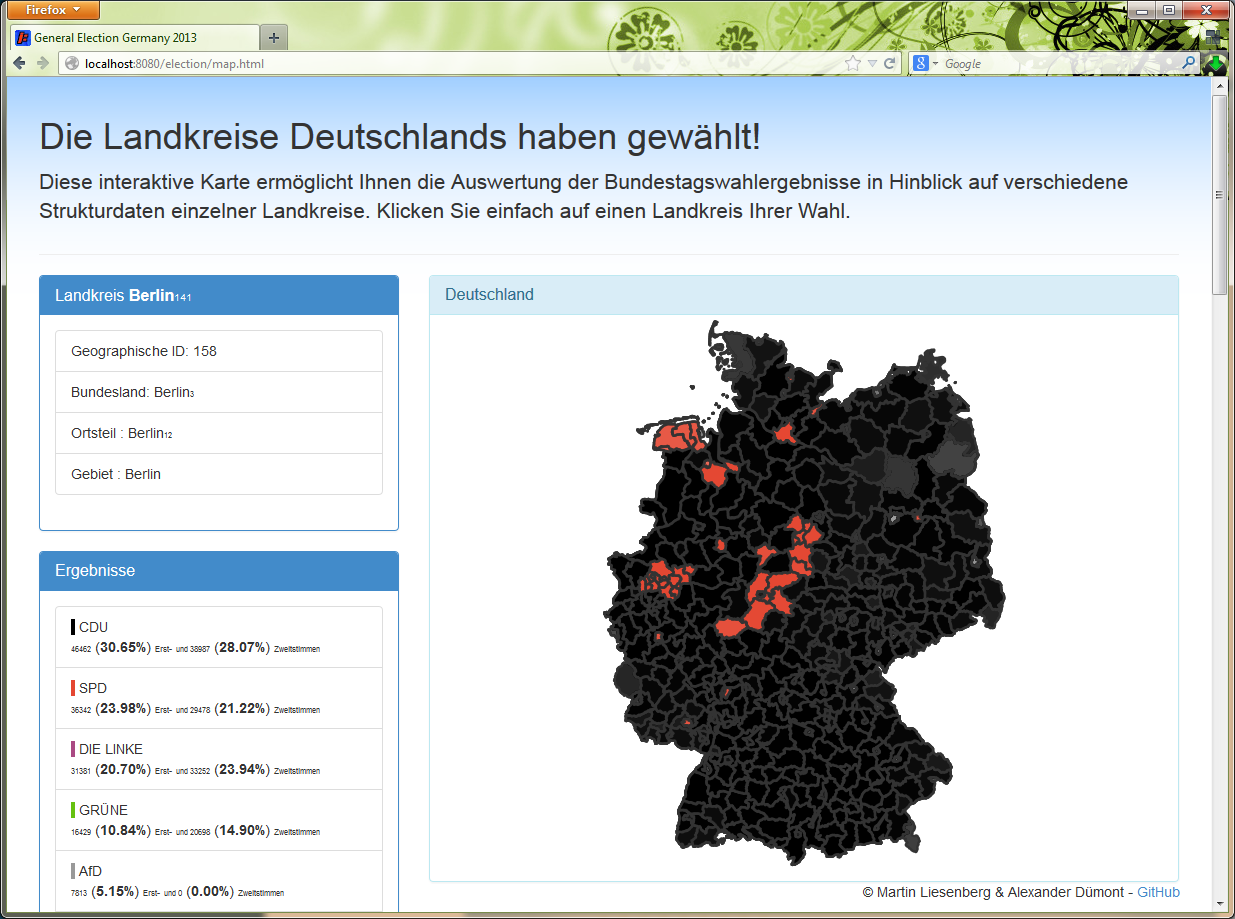
\includegraphics[width=1.2\textwidth]{../img/JKGj20F.png}
\caption{Browser Screenshot}
\end{figure}


\section{Description}

\subsubsection{Task}\label{task}

The goal of the project is to work with the data of the German federal
election from 2013 and spatial map data of Germany from the Global
Administrative Areas.

\subsubsection{Requirements}\label{requirements}

Find sources for
\begin{itemize}
\item
  detailed results of each state,
\item
  shape files of the constituencies and
\item
  data to combine with the election results
\end{itemize}

Model your data in ER and store the data in PostGIS\\Overlay the
administrative borders of each state and the constituencies\\Visualize
the results of the election on the map

\subsubsection{Result}\label{result}

We built a web based application connecting statistical data with the
results of the federal election based on a PostgreSQL database with a
PostGIS extension. The primary programming language for the backend is
Java, for the frontend it's Javascript.

\subsubsection{Wiki Overview}\label{wiki-overview}

The wiki is meant to give an overview of the application describing
general concepts used in the development and pointing out interesting
features and solution.\\The first part is focussed on the data sources,
the second part deals with the actual implementation.


\section{Strategy}

\begin{enumerate}
\def\labelenumi{\arabic{enumi}.}
\itemsep1pt\parskip0pt\parsep0pt
\item
  AngularJS
\item
  Twitter Bootstrap
\item
  d3.js
\item
  hibernate.spatial
\item
  Maven
\end{enumerate}

\subsubsection{1.
\href{http://angularjs.org/}{\textbf{AngularJS}}}\label{angularjs}

AngularJS is an open source JavaScript MVC (model-view-controller)
Framework maintained by Google for writing dynamic web applications. It
offers the possibility to extend the standard HTML language, two-way
data binding and dependency injection. For a more detailed introduction
see the \href{http://docs.angularjs.org/guide/introduction}{AngularJS}
documentation.

\subsubsection{2.
\href{http://getbootstrap.com/components/}{\textbf{Twitter
Bootstrap}}}\label{twitter-bootstrap}

Twitter Bootstrap is an open source collection of tools for web
development. It comprises of a number of HTML and CSS based design
templates for buttons, forms, navigation etc and a number of JavaScript
dependant dynamic extensions. See the
\href{http://getbootstrap.com/}{website} for details.

\subsubsection{3. \href{http://d3js.org/}{\textbf{d3.js}}}\label{d3.js}

d3.js is a JavaScript library using HTML, CSS and SVG to visualize data.
It uses pre-built JavaScript functions to select elements, create SVG
objects, style them, or add transitions, dynamic effects or tooltips to
them. The objects can also be styled using CSS. Datasets can be bound to
SVG objects using simple D3 functions to generate graphics.

\subsubsection{4.
\href{http://www.hibernatespatial.org/}{\textbf{Hibernate
Spatial}}}\label{hibernate-spatial}

Hibernate Spatial is an extension to Hibernate to handle geographic
data. It uses the Java Topology Suite as its geometry model. JTS is an
implementation of the OpenGIS Simple Features Implementation
Specification for SQLv. 1.1 (SFS). This specification is implemented in
most RDBMS with spatial data support. It is also a direct precursor to a
precursor to SQL/MM Part 3: Spatial (ISO/IEC 13249-3).

\subsubsection{5. \href{http://maven.apache.org/}{\textbf{Apache
Maven}}}\label{apache-maven}

Apache Maven is a software project management tool. Based on the concept
of a project object model (POM), Maven can manage a project's build,
reporting and documentation from a central source repository. In our
project is used for dependency and build management.


\section{Database Model}

\begin{enumerate}
\def\labelenumi{\arabic{enumi}.}
\itemsep1pt\parskip0pt\parsep0pt
\item
  General Approach
\item
  Implementation
\end{enumerate}

\subsubsection{General Approach}\label{general-approach}

\begin{figure}[htbp]
\centering
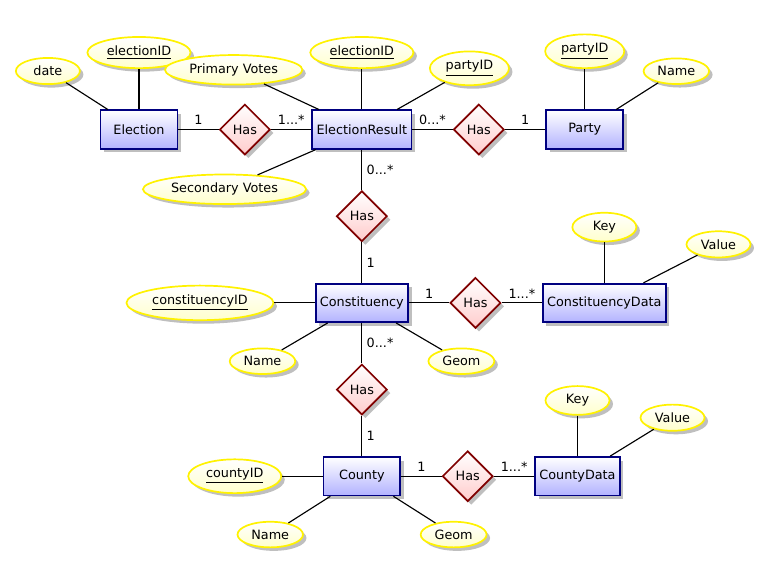
\includegraphics[width=1.1\textwidth]{../img/KIQu2J3.png}
\caption{uml}
\end{figure}

\subsubsection{Implementation}\label{implementation}

\textbf{Election Results}
\\Constituency 1\textless{}-\textgreater{}n
ElectionResult n\textless{}-\textgreater{}1
Party
\\ElectionResult(Constituency\_ID, Party\_ID, election\_ID,
primaryVotes, secondaryVotes)



\begin{lstlisting}
CREATE TABLE electionresult
(
  constituencyid integer NOT NULL,
  partyid integer NOT NULL,
  primaryVotes integer,
  secondaryVotes integer,
  election_electionid bigint,
  CONSTRAINT constituency_fk FOREIGN KEY (constituencyid)
      REFERENCES constituency (gid) MATCH SIMPLE
      ON UPDATE NO ACTION ON DELETE NO ACTION,
  CONSTRAINT election_fk FOREIGN KEY (election_electionid)
      REFERENCES election (electionid) MATCH SIMPLE
      ON UPDATE NO ACTION ON DELETE NO ACTION,
  CONSTRAINT party_fk FOREIGN KEY (partyid)
      REFERENCES party (partyid) MATCH SIMPLE
      ON UPDATE NO ACTION ON DELETE NO ACTION
)
\end{lstlisting}

\textbf{Party}
\\Party(Party\_ID, Name)


\begin{lstlisting}
CREATE TABLE party
(
  partyid serial NOT NULL,
  name character(200),
  color character varying(255),
  partyname character varying(255),
  CONSTRAINT party_pkey PRIMARY KEY (partyid)
)
\end{lstlisting}


\textbf{Election}
\\Election(election\_ID, date, year)
Election(election\_ID, date, year)

\begin{lstlisting}
CREATE TABLE election
(
  electionid bigint NOT NULL,
  date timestamp without time zone,
  year integer NOT NULL,
  CONSTRAINT election_pkey PRIMARY KEY (electionid)
)
\end{lstlisting}

\textbf{Constituency Data}
\\Constituency 1\textless{}-\textgreater{}n
ConstituencyData n \textless{}-\textgreater{} 1 ConstituencyDataKeys
ConstituencyData(Constituency\_ID, Key\_ID,
Value)\\ConstituencyDataKeys(Key\_ID, name)



\begin{lstlisting}
CREATE TABLE public.constituency_data
(
  gid BIGINT NOT NULL,
  key CHARACTER VARYING(255),
  value BIGINT NOT NULL,
  CONSTRAINT belongs_to_constituency FOREIGN KEY (gid)
      REFERENCES constituency (gid) MATCH SIMPLE
      ON UPDATE NO ACTION ON DELETE NO ACTION
)
\end{lstlisting}

\textbf{County Data}
\\County 1 \textless{}-\textgreater{} n CountyData n \textless{}-\textgreater{}
1 CountyDataKeys CountyData(County\_ID, Key\_ID, Value)
\\CountyDataKeys(Key\_ID, name)

\begin{lstlisting}
CREATE TABLE public.county_data
(
  gid BIGINT NOT NULL,
  key CHARACTER VARYING(255),
  value BIGINT NOT NULL,
  CONSTRAINT belongs_to_county FOREIGN KEY (gid)
      REFERENCES county (gid) MATCH SIMPLE
      ON UPDATE NO ACTION ON DELETE NO ACTION
)
\end{lstlisting}

\textbf{County}
\\County(County\_ID, Name, Nr, coordinates)

\textbf{Constituency}
\\Constituency(Constituency\_ID, Name, Nr,
coordinates)


\section{Database Layer}

\begin{enumerate}
\def\labelenumi{\arabic{enumi}.}
\itemsep1pt\parskip0pt\parsep0pt
\item
  Hibernate
\item
  Data Access Object
\item
  JAX-RS API 2.0
\end{enumerate}

\subsubsection{1. Hibernate}\label{hibernate}

Hibernate is an open source persistence and ORM framework for Java. It
is being used to map Java classes to database tables and provides means
to query and retrieve data without writing SQL.\\The mapping is done via
annotations which is being used for attributes as well as relations
between entities (many-to-one, many-to-many, etc.). In order for
Hibernate to manage the persistence, the class has to provide a no
arguments constructor. We used an extension to Hibernate called
Hibernate Spatial which also provides support for spatial data types
such as Point and MultiPolygon. Find an example below:


\begin{lstlisting}
@Id // indicating the primary key
@GeneratedValue(strategy=GenerationType.SEQUENCE) // how is the key generated
private long gid;

@Column(unique=true) // enforce unique constraint on column
private int wkr_nr;

// spatial type using extended annotations provided by hibernate spatial
@Type(type="org.hibernate.spatial.GeometryType")
@Column(columnDefinition="Geometry")
private Point centerPoint;

// ...

// defining a 1 <-> n relation between constituency and county
@OneToMany(fetch=FetchType.LAZY)
@JoinColumn(name="constituency_id", referencedColumnName="wkr_nr")
@OrderBy("areaQuota")
private List<CountyContainsConstituency> dependingCounties = new LinkedList<CountyContainsConstituency>();

// ...
\end{lstlisting}


\subsubsection{2. Data Access Object}\label{data-access-object}

\begin{figure}[htbp]
\centering
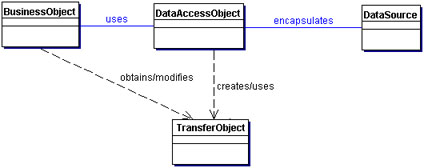
\includegraphics[width=0.9\textwidth]{../img/146804.jpg}
\caption{Data Access Object UML Diagram by Oracle (Core J2EE Patterns)}
\end{figure}

The pattern is used to provide a layer of abstraction between the actual
data source and the application logic using the data. By defining a
couple of interfaces and providing different implementing classes for
the different data sources changing the data source of an application
becomes rather easy. Below a UML diagram of our DAO classes.

\begin{figure}[htbp]
\centering
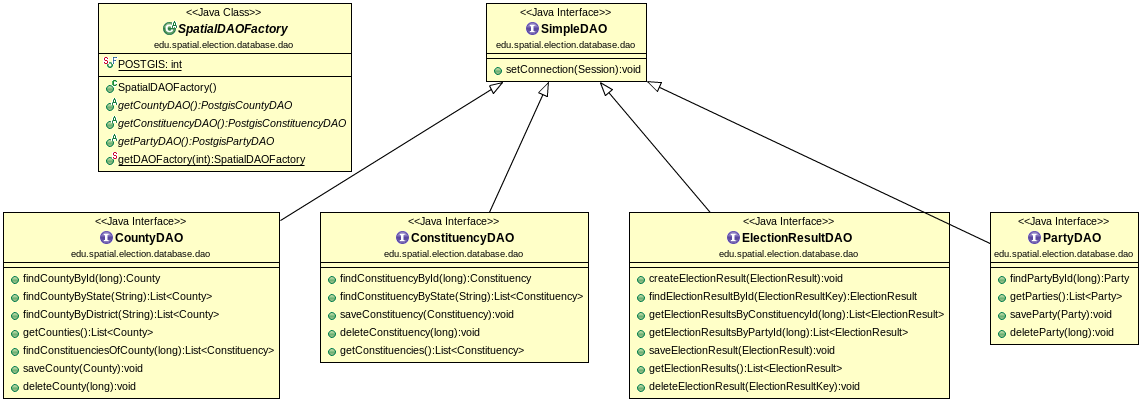
\includegraphics[width=1.2\textwidth]{../img/6CeJf06.png}
\caption{Class Diagramm}
\end{figure}

\textbf{Thoughts on using the pattern}\\Though it might seem a little
bit over the top to use such a rather complex structure for a small
scale project, we deemed it good software engineering practice to
separate data access from application logic. Moreover if a follow up
project wants to measure the performance of different databases while
using the application or simply decides to switch the underlying
database they simply need to implement another set of Data Access Object
classes.

\subsubsection{3. JAX-RS API 2.0}\label{jax-rs-api-2.0}

With the help of JAX-RS plain Java Objects can be exposed as RESTful Web
resources independent of the underlying technology using a declarative
and annotation based API.

\begin{lstlisting}
@Path("/constituency")
public class RestConstituency \{
    private SpatialDAOFactory f = SpatialDAOFactory.getDAOFactory(SpatialDAOFactory.POSTGIS);

	// ...
	
    @GET
    @Path("{id}/geometry")
    @Produces({MediaType.APPLICATION_JSON})
    public double[][][] getConstituencyGeometryById(@PathParam("id") long id)
    \{ Session s = DatabaseConnection.openSession();
        // Create a DAO
        ConstituencyDAO constituencyDAO = f.getConstituencyDAO();
        constituencyDAO.setConnection(s);

	Constituency c = constituencyDAO.findConstituencyById(id);
	c.setGeometryDetail(0);
	c.getGeometryArray();
	double[][][] result = c.getGeometryArray();
		
	s.close();
	return result;
    \}
    
	// ...
\}
\end{lstlisting}

\texttt{@Path} specifies the relative path of the function,
\texttt{@GET} the type of method (\texttt{@POST}, \texttt{@DELETE} and
\texttt{@PUT} are also available) and
\texttt{@Produces(\{MediaType.APPLICATION\_JSON\})} indicates that the
method will eventually return JSON (as opposed to \texttt{@Consumes}
which indicates that the method is passed a particular type).\\Another
interesting feature to note is \texttt{@PathParam} which is being passed
to the function. It's used to identify a single instance of a
constituency and binds the method parameter to a path segment.


\section{Constituencies and Counties}

\begin{enumerate}
\def\labelenumi{\arabic{enumi}.}
\itemsep1pt\parskip0pt\parsep0pt
\item
  About Wahlkreise and Landkreise
\item
  Configuration and Visualization in QGIS Desktop
\item
  Setup for Postgres (+Postgis)
\item
  Derivation of \emph{County} \textless{}-\textgreater{}
  \emph{Constituency}
\end{enumerate}

\subsection{1. About Wahlkreise and
Landkreise}\label{about-wahlkreise-and-landkreise}

\emph{{[}Description{]}}

\subsection{2. Configuration and Visualization in QGIS
Desktop}\label{configuration-and-visualization-in-qgis-desktop}

\subsubsection{Requirements}\label{requirements}

Available Layers *
\href{http://www.bundeswahlleiter.de/en/bundestagswahlen/BTW_BUND_13/wahlkreiseinteilung/kartographische_darstellung.html}{Wahlkreise}
* Download:
\href{http://www.bundeswahlleiter.de/de/bundestagswahlen/BTW_BUND_13/wahlkreiseinteilung/wahlkreisgeometrie/Geometrie_Wahlkreise_18DBT_VG1000_ETRS89.zip}{SHP}
* Projection: \textbf{EPSG:3044 - ETRS89 / ETRS-TM32} *
\href{http://www.gadm.org/country}{Landkreise} * Download
\href{http://biogeo.ucdavis.edu/data/gadm2/shp/DEU_adm.zip}{SHP} *
Projection: \textbf{EPSG:4326 - WGS84}

\subsubsection{Visualization}\label{visualization}

\begin{figure}[htbp]
\centering
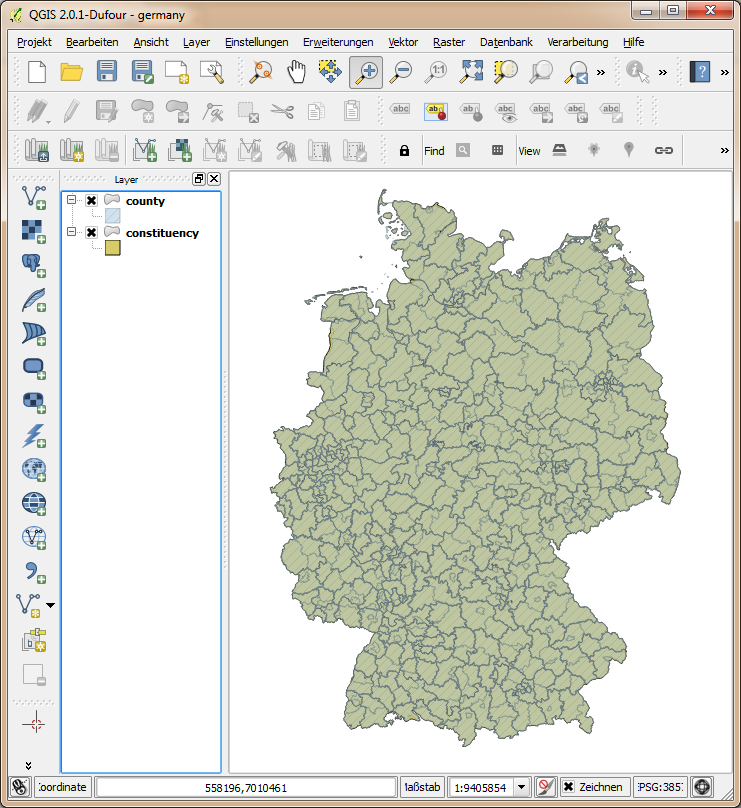
\includegraphics[width=1.1\textwidth]{../img/K4GjcyV.png}
\caption{WahlkreiseNLandkreise1}
\end{figure}

\subsubsection{Issues}\label{issues}

\begin{figure}[htbp]
\centering
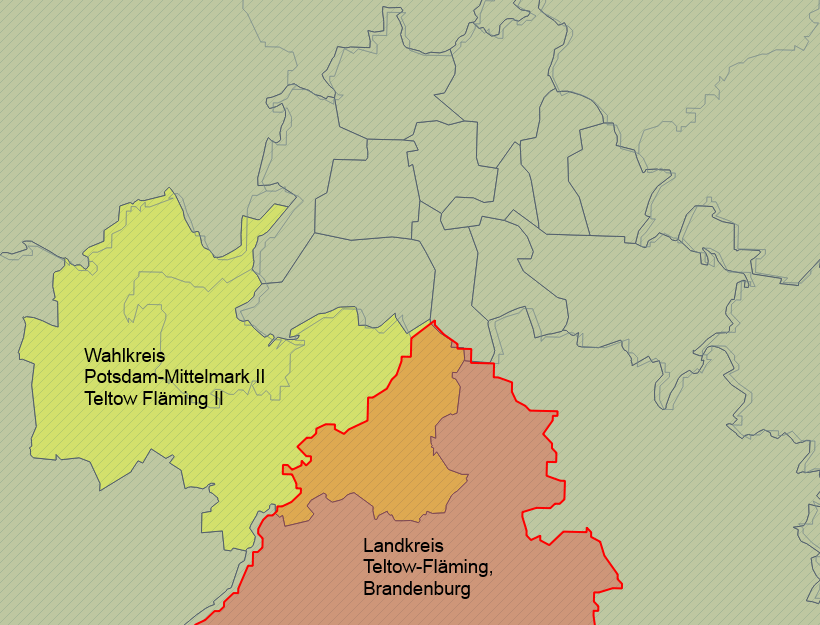
\includegraphics[width=1.1\textwidth]{../img/HdnNLcV.png}
\caption{WahlkreisVLandkreis}
\end{figure}

\begin{enumerate}
\def\labelenumi{\arabic{enumi}.}
\itemsep1pt\parskip0pt\parsep0pt
\item
  \emph{Wahlkreise} and \emph{Landkreise} are not dependent, thus their
  areas are freely intersecting each other.
\item
  \emph{Wahlkreise} and \emph{Landkreise} show a different degree of
  accuracy in position and detail when it comes to border polygons.
\end{enumerate}

\subsection{3. Setup for Postgres
(+Postgis)}\label{setup-for-postgres-postgis}

\begin{enumerate}
\def\labelenumi{\arabic{enumi}.}
\itemsep1pt\parskip0pt\parsep0pt
\item
  Import shapefiles to the database \emph{public} schema.
\end{enumerate}

\begin{itemize}
\itemsep1pt\parskip0pt\parsep0pt
\item
  \emph{Landkreise} -\textgreater{} ``county''
\item
  \emph{Wahlkreise} -\textgreater{} ``constituency''
\end{itemize}

\begin{enumerate}
\def\labelenumi{\arabic{enumi}.}
\setcounter{enumi}{1}
\itemsep1pt\parskip0pt\parsep0pt
\item
  Add two materialized SQL-Views (virtual tables) for intersections /
  dependencies between ``county'' and ``constituency'':
\end{enumerate}

\begin{lstlisting}
-- delete old view
DROP MATERIALIZED VIEW IF EXISTS public.county_intersecting_constituency;

-- create area intersection view
CREATE MATERIALIZED VIEW public.county_intersecting_constituency AS 

 WITH intersections AS (
  SELECT lk.id_3 AS county_id,
	wktrns.wkr_nr AS constituency_id,
	CONCAT(lk.name_3, ' (', lk.name_1, ', ', lk.name_2, ')') AS county_label,
	wktrns.wkr_name AS constituency_label,
	ST_AREA(ST_INTERSECTION(ST_SetSRID(lk.geom,4326), wktrns.shape)::geography) AS area_intersection,
	ST_AREA(ST_SetSRID(lk.geom,4326)::geography) AS area_county,
	ST_AREA(wktrns.shape::geography) AS area_constituency
  FROM
	county lk
	JOIN (select wkr_nr, wkr_name, ST_Transform(ST_SetSRID(geom,3044), 4326) AS shape FROM constituency) AS wktrns
	ON ST_INTERSECTS(ST_SetSRID(lk.geom,4326), wktrns.shape))
	
 SELECT
	county_id,
	constituency_id,
	county_label,
	constituency_label,
	area_intersection,
	area_intersection / ((SELECT SUM(i.area_intersection) FROM intersections i WHERE i.county_id = intersections.county_id)) AS area_quota,
	area_county,
	area_constituency
 FROM intersections;

CREATE UNIQUE INDEX county_intersecting_constituency_unique
  ON public.county_intersecting_constituency (county_id, constituency_id);
\end{lstlisting}

\subsection{4. Derivation of \emph{County} \textless{}-\textgreater{}
\emph{Constituency}}\label{derivation-of-county---constituency}

Take \emph{Berlin} for example:

\begin{lstlisting}
select * from county_intersecting_constituency where county_label like '%Berlin%' order by area_intersection;
\end{lstlisting}

This request results in a join of intersecting counties and
constituencies, with information about the area of the participate
county, constituency and of course the intersection. A normalized
intersection \textbf{``quota''} index is calculated, which defines the
areal influence of a constituency to a county. The sum of all
constituency ``quota'' of a county is 1.

\begin{table}[h]
\scalebox{0.5}{
\begin{tabular}{|c|c|l|l|r|r|r|r|}
\hline\textbf{county\_id} & \textbf{constituency\_id} & \textbf{county\_label} & \textbf{constituency\_label} & \textbf{area\_intersection} & \textbf{area\_quota} & \textbf{area\_constituency} & \textbf{area\_county} \\ \hline 
141	  &	58    		 &	"Berlin"     &	"Oberhavel Havelland II"	 &	  2803665.490080   &	0.00316685814074   &	2472931758.37186   &	885316816.471166 \\ 
141	  &	63    		 &	"Berlin"     &	"Frankfurt (Oder) Oder-{[}...{]}"   &	  5752379.328977   &	0.00649755449466   &	2405885789.94363   &	885316816.471166 \\ 
141	  &	61    		 &	"Berlin"     &	"Potsdam Potsdam-Mittel{[}...{]}"   &	  6948676.937887   &	0.00784882298049   &	 727030312.23901   &	885316816.471166 \\ 
141	  &	62    		 &	"Berlin"     &	"Dahme-Spreewald Teltow{[}...{]}"   &	  8343997.350849   &	0.00942489609776   &	3973353611.91130   &	885316816.471166 \\ 
141	  &	59    		 &	"Berlin"     &	"M\"arkisch-Oderland Barn{[}...{]}"   &	  8982614.974483   &	0.01014624157473   &	2864879802.60181   &	885316816.471166 \\ 
141	  &	83    		 &	"Berlin"     &	"Berlin-Friedrichshain-K{[}...{]}"   &	 28018823.320075   &	0.03164843988671   &	  28018823.32007   &	885316816.471166 \\ 
141	  &	75    		 &	"Berlin"     &	"Berlin-Mitte"			 &	 45474155.779447   &	0.05136497236676   &	  45474155.77944   &	885316816.471166 \\ 
141	  &	82    		 &	"Berlin"     &	"Berlin-Neuk\"olln"	   	 &	 50038162.639312   &	0.05652021015447   &	  51552590.88985   &	885316816.471166 \\ 
141	  &	81    		 &	"Berlin"     &	"Berlin-Tempelhof-Sch\"one{[}...{]}"   &	 50911846.188703   &	0.05750707248545   &	  52138379.69080   &	885316816.471166 \\ 
141	  &	86    		 &	"Berlin"     &	"Berlin-Lichtenberg"		 &	 54387933.428961   &	0.06143345928648   &	  54578186.82576   &	885316816.471166 \\ 
141	  &	85    		 &	"Berlin"     &	"Berlin-Marzahn-Hellersd{[}...{]}"   &	 55587278.018553   &	0.06278816946519   &	  56213685.87850   &	885316816.471166 \\ 
141	  &	80   		 &	"Berlin"     &	"Berlin-Charlottenburg-W{[}...{]}"   &	 64557831.259508   &	0.07292078680438   &	  64557831.25950   &	885316816.471166 \\ 
141	  &	78   		 &	"Berlin"     &	"Berlin-Spandau Charlot{[}...{]}"   &	 70910610.225396   &	0.08009651795193   &	  83642855.89283   &	885316816.471166 \\ 
141	  &	77    		 &	"Berlin"     &	"Berlin-Reinickendorf"		 &	 77263528.269943   &	0.08727240619467   &	  84103703.05926   &	885316816.471166 \\ 
141	  &	76    		 &	"Berlin"     &	"Berlin-Pankow"			 &	 90999372.170865   &	0.10278761984321   &	  95504666.59105   &	885316816.471166 \\ 
141	  &	79    		 &	"Berlin"     &	"Berlin-Steglitz-Zehlend{[}...{]}"   &	102307387.695839   &	0.11556049918550   &	 106561169.57164   &	885316816.471166 \\ 
141	  &	84    		 &	"Berlin"     &	"Berlin-Treptow-K\"openick"	 &	162026255.436742   &	0.18301547308679   &	 167319473.44736   &	885316816.471166 \\  \hline 
             
\end{tabular}
}
\end{table}


\emph{Notice:} Since the map data of constituencies and counties are
inaccurately overlapping a part of \emph{Brandenburg} constituencies
intersect with the county \emph{Berlin}. The sum of all
\textbf{``quota''} from \emph{Brandenburg} constituencies in
\emph{Berlin} county is 0.03708, which means 3.7\% of \emph{Berlin}s
area will be influenced by voting results descending from constituency
of \emph{Brandenburg}.




\section{Frontend}

The frontend can be described best by giving general information about:

\begin{enumerate}
\def\labelenumi{\arabic{enumi}.}
\itemsep1pt\parskip0pt\parsep0pt
\item
  Structuring the page
\item
  Building the map
\item
  Getting the data
\end{enumerate}

\subsection{Structuring the page}\label{structuring-the-page}

As mentioned in the Frameworks Section
we used the Twitter Bootstrap Framework to desgin our application.
Though responsive design is not a priority, the framework does provide
easy to use abstractions to structure a page, plus makes it easy to
stick to a coherent design.

By providing HTML tags with predefined class attributes Bootstrap
enables its user to easily enhance his/her application. The following
snippet divides the page horizontally in two sections, one a third of
the total width, the other two thirds.


\begin{lstlisting}[language=HTML]
<div class="row">
	<div class="col-md-4">
        .....
        </div>
	<div class="col-md-8">
        ....
        </div>
</div>
\end{lstlisting}



\subsection{Building the map}\label{building-the-map}

Within the main div tag of the page the map is displayed.



\begin{lstlisting}[language=HTML]
<div class="panel-body" style="padding:0px">
    <div id="mysvg"></div>
</div>
\end{lstlisting}


As described elsewhere the data to be displayed is loaded on startup
with a call to the REST API provided by our backend.

First a \emph{svg} element and a projection are created.

\begin{lstlisting}
var vis = d3.select("#mysvg").append("svg:svg").attr("width", width).attr("height", height); 
var projection = d3.geo.mercator().center([10.45, 51.30]).scale(2500).translate([width/2,height/2]);
\end{lstlisting}


Later all counties are added to this element. Additionally, a zoom
handler (displayed below) and a click handler are added to look closer
at a county and to display the extrapolated data in the column next to
the map. All counties are colored according to the party who won the
majority of the vote.


\begin{lstlisting}
var zooming = false;
var zoom = d3.behavior.zoom().scaleExtent([1, 8])
  .on("zoom", function() {
    if(!zooming) {
        doclick = false;
        zooming = true;
        var scale = d3.event.scale;
        var trans = scale == 1 ? "0.0, 0.0" : d3.event.translate;
        g.attr("transform", "translate(" + trans + ") scale(" + scale + ")");
        features.attr("stroke-width", strokeWidth(scale) + "");
        zooming = false;
    }
});
var g = vis.append("g").call(zoom);
\end{lstlisting}


\subsubsection{Getting the data}\label{getting-the-data}

The data is provided by calls to the RESTful API of the application. For
each class of entities we need we defined a \emph{factory} encapsulating
a \emph{resource} object, a service from the
\href{http://docs.angularjs.org/api/ngResource}{\emph{ngResource}}
module as provided by AngularJS. Through the object returned by the
factory one can conveniently execute \emph{get}, \emph{post}, \emph{put}
and \emph{delete} requests. For our use case \emph{get} is normally
enough. An example implementation is shown below.



\begin{lstlisting}
angular.module('myApp.services', ['ngResource'])
.factory('Counties', [ '$resource',
  function($resource) {
	var baseurl = 'backend/county/votes/';
	return $resource(baseurl + ':level/', {
		id : '@level'
	},
    {
        'get': {
            method: 'GET',
            transformResponse: function (data) {
            	var dat = angular.fromJson(data);
            	return dat.list ? dat.list : dat;
            },
            isArray: true
        }
    });
}])
\end{lstlisting}

A \emph{get} request is dispatched as follows. First the factory is
injected into the controller which is using it by passing it as an
argument, then a simple function invocation is made.



\begin{lstlisting}
// simplified example
angular.module('myApp.controllers', [])
.controller('mapCtrl', function mapCtrl($scope, Counties, ...) {
	Counties.get({'level' : 2}).$promise.then(function(counties) {
		displayWahlkreise(counties);
	});
});
\end{lstlisting}





\section{Setup Eclipse}

Setting up a Maven multiple-project hierarchy is not difficult. All it
takes are 6 easy steps:

\begin{enumerate}
\def\labelenumi{\arabic{enumi}.}
\item
  Download and install the
  \href{https://www.eclipse.org/downloads/}{Eclipse}-IDE (integrated
  development environment), if you don't have already. You can use the
  standard edition.
\item
  Download and unzip the newest
  \href{https://github.com/a-d/spatial.election/archive/master.zip}{spatial.election}
  files.
\item
  Start Eclipse, see figure \ref{eclipse01}.
  
  \begin{figure}[htbp]
  \centering
  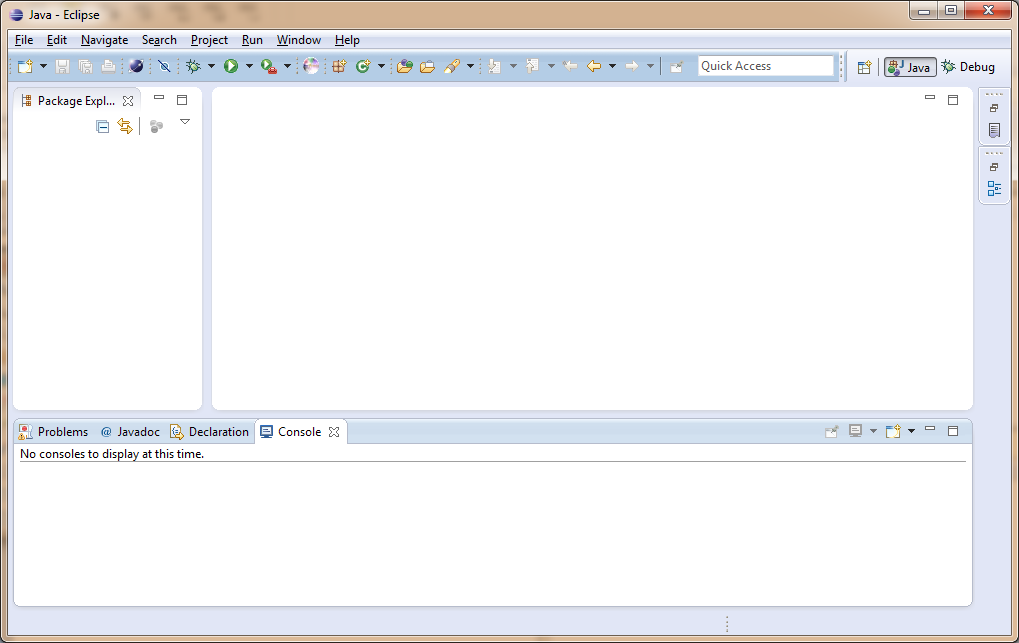
\includegraphics[width=1.1\textwidth]{../img/GMXSI1f.png}
  \caption{Eclipse Startup}
  \label{eclipse01}
  \end{figure}
  
\item
  Check whether M2E is installed. It's a plugin for eclipse, providing
  Maven features. Go to \textbf{Help} -\textgreater{} \textbf{Install
  New Software}. Enter the site ``\textbf{M2E -
  !http://download.eclipse.org/technology/m2e/releases}''. Install
  ``Maven Integration for Eclipse'' if it is not yet installed. Restart
  Eclipse if necessary. See figure \ref{eclipse02}. \\

  \begin{figure}[htbp]
  \centering
  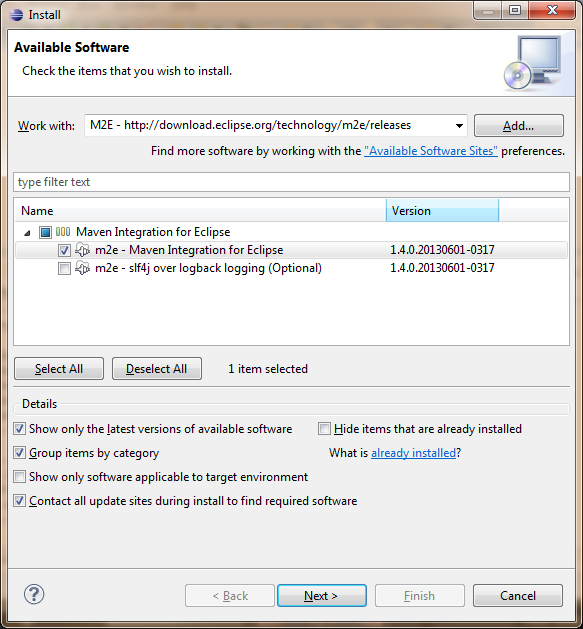
\includegraphics[width=1.1\textwidth]{../img/nO8HPxH.png}
  \caption{Eclipse M2E installation}
  \label{eclipse02}
  \end{figure}
\item
  Import the \emph{spatial.election} project, by using \textbf{File}
  -\textgreater{} \textbf{Import}, check ``Existing Maven Projects''. See figure
  \ref{eclipse03}.
  
  \begin{figure}[htbp]
  \centering
  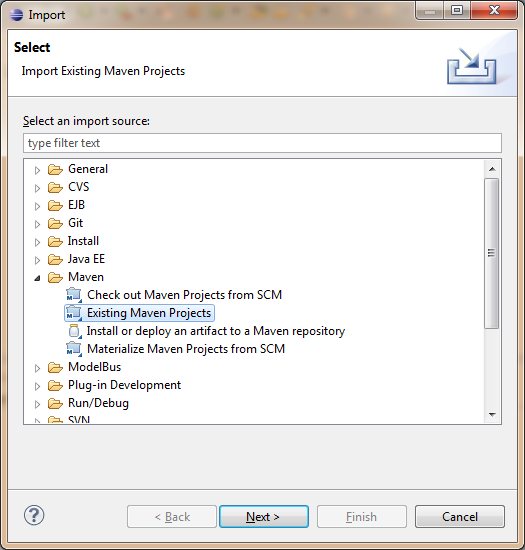
\includegraphics[width=1.1\textwidth]{../img/OozCHLd.png}
  \caption{Eclipse project import}
  \label{eclipse03}
  \end{figure}
\item
  Enter the path to your unziped \emph{spatial.election} files. Check
  all projects and skip through the following \emph{Import} dialogs.
   See figure \ref{eclipse04}.
   
  \begin{figure}[htbp]
  \centering
  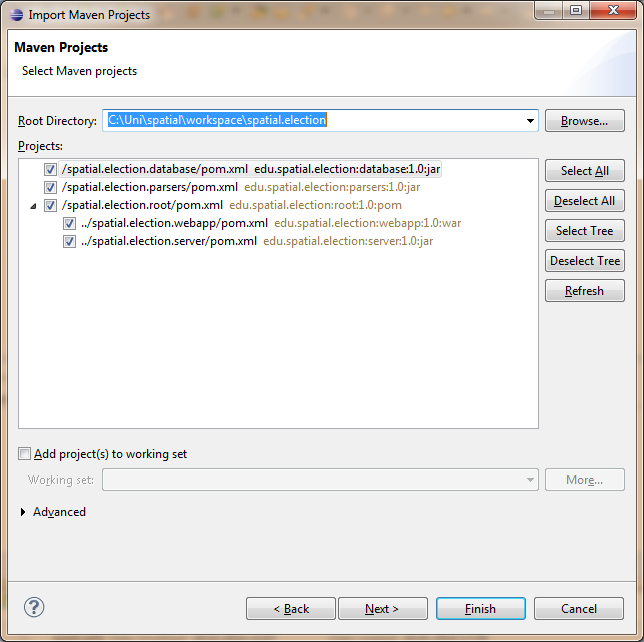
\includegraphics[width=1.1\textwidth]{../img/vBZ4xNA.png}
  \caption{Eclipse path and project selection}
  \label{eclipse04}
  \end{figure}
\end{enumerate}

\begin{center}\rule{3in}{0.4pt}\end{center}

Now Eclipse is ready to use the
\emph{spatial.election} software with source code, see figure \ref{eclipse05}
The code can be altered, as well as build and run as application. If the Setup
of PostgreSQL server is already done, the software is ready to run.

\begin{figure}[htbp]
\centering
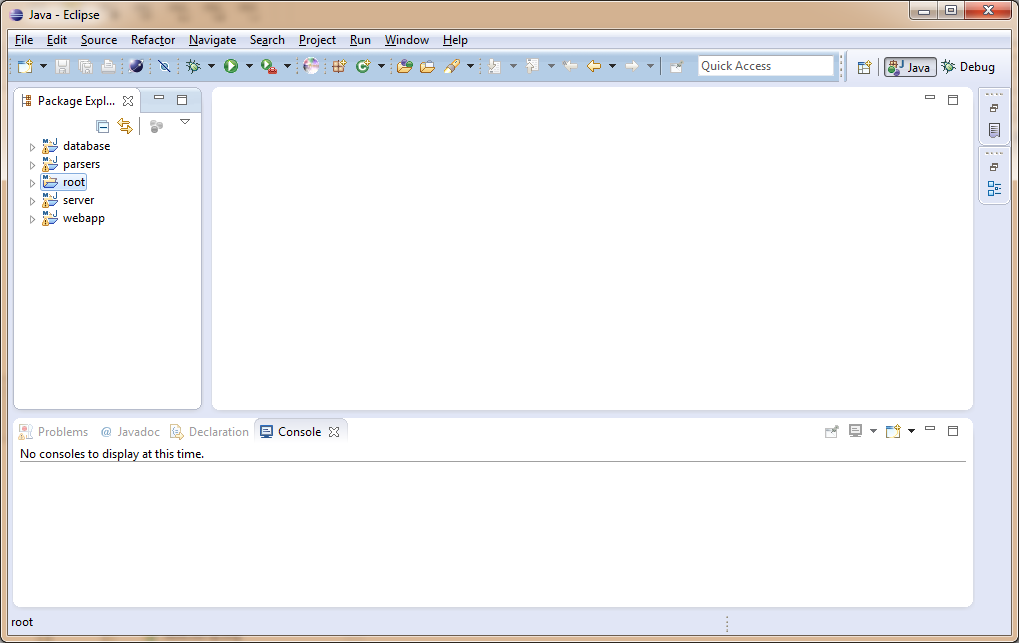
\includegraphics[width=1.1\textwidth]{../img/EeGnXjg.png}
\caption{Eclipse complete setup}
\label{eclipse05}
\end{figure}


\section{Setup Postgres}

A valid PostgreSQL environment including PostGIS can be set up by
following the two steps:

\begin{enumerate}
\def\labelenumi{\arabic{enumi}.}
\item
  Visit the \href{http://www.postgresql.org/}{PostgreSQL website} and
  download the current version. (e.g. \textbf{9.3})
\item
  Visit the \href{http://postgis.net/}{PostGIS website} and download the
  current version. (e.g. \textbf{2.1})
\end{enumerate}

If a Debian system is running, installing a
precompiled version is recommend. In that case, follow the
\href{https://wiki.postgresql.org/wiki/Apt}{official instructions} to do
so. As soon as the postgres related APT pgdg repository is registered,
the following command can be run:

\begin{lstlisting}[numbers=none, language=bash]
$ apt-get install postgresql-server-dev-9.3 postgresql-9.3-postgis-2.1
\end{lstlisting}

If you are running a Windows system and you are asked to whether or not
insall plugins, during the installation process; feel free to install
the delivered PostGIS plugin. It may not be the newest version, but it
will suffice.

\subsection{Importing the Database}\label{importing-the-database}

\begin{enumerate}
\def\labelenumi{\arabic{enumi}.}
\item
  To import the database, you need to first create a database:

\begin{lstlisting}[numbers=none, language=bash]
$ createdb spatial_election --encoding UNICODE --template=template0
$ psql spatial_election
> CREATE EXTENSION postgis;
> CREATE EXTENSION postgis_topology;   
> \q
\end{lstlisting}
\item
  Then you need to restore the database dump file to your database. You
  need to dowmload the
  \href{https://github.com/a-d/spatial.election/raw/master/spatial.election.data/spatial_db.backup}{spatial\_db.backup
  file}.

\begin{lstlisting}[numbers=none, language=bash]
$ pg_restore -d spatial_election spatial_db.backup
\end{lstlisting}

\item
  Create a role with password according to
  \href{https://github.com/a-d/spatial.election/blob/master/spatial.election.database/src/main/resources/hibernate.cfg.xml}{your
  hibernate.cfg.xml}
\end{enumerate}


\section{Running}


There are 3 different ways to run the application. But first open up
Eclipse, which has been previously have set
up.

\subsection{Debugging inside of
Eclipse}\label{debugging-inside-of-eclipse}

\begin{enumerate}
\def\labelenumi{\arabic{enumi}.}
\item
  Create a \emph{Run Configuration} with ``jetty:run'' as goal for the
  \emph{webapp} project. See figure \ref{run01}.
  
\item
  Save configuration and run it. If the program runs properly the
  console should look something like in figure \ref{run02}.
\item
  Use your browser to open http://localhost:8080/election
\end{enumerate}

\begin{figure}[htbp]
\centering
  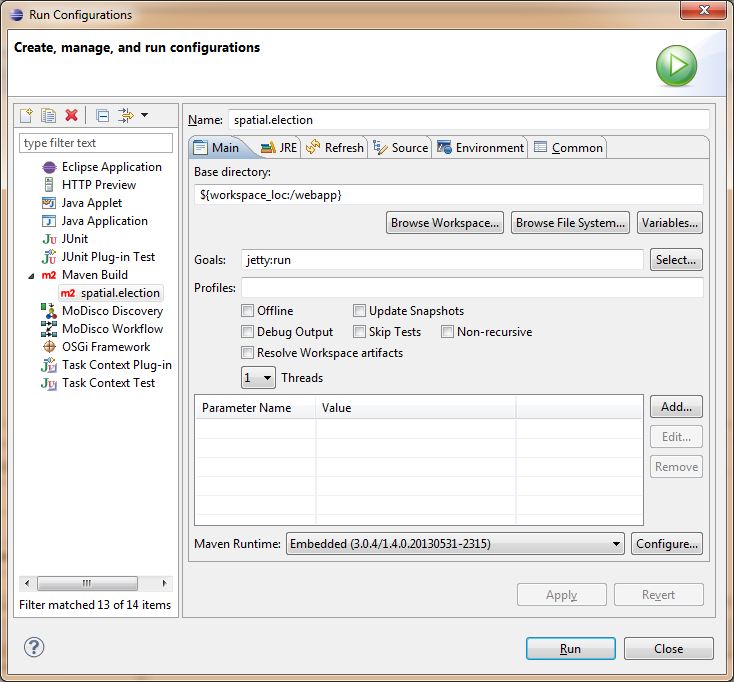
\includegraphics[width=1.1\textwidth]{../img/dwACYmd.png}
\caption{Eclipse run configuration}
\label{run01}
\end{figure}

\begin{figure}[htbp]
\centering
  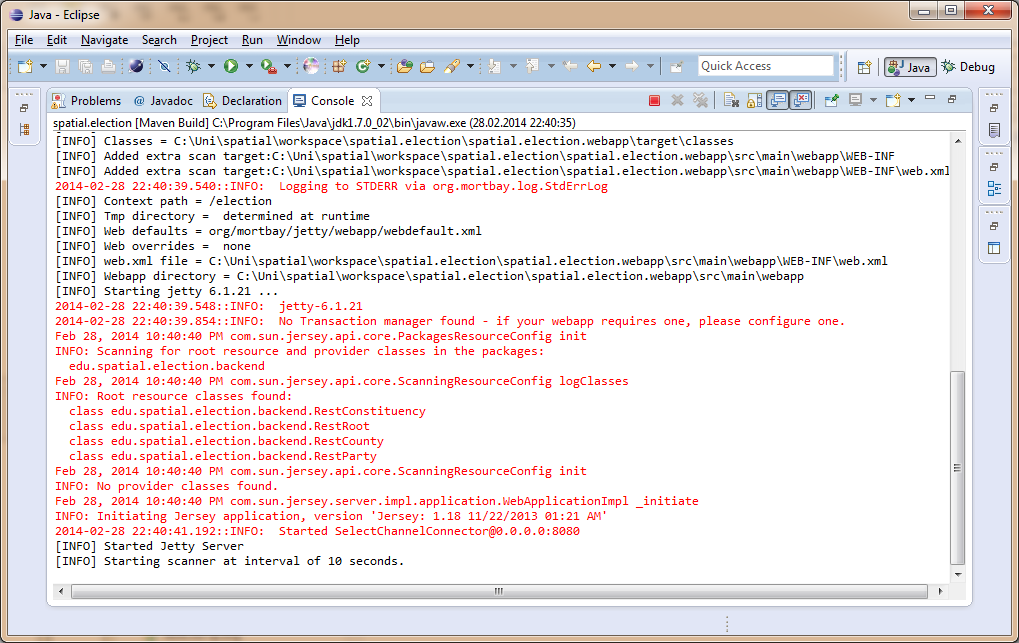
\includegraphics[width=1.1\textwidth]{../img/UZXVJIp.png}
\caption{Eclipse project run in Console view}
\label{run02}
\end{figure}

\begin{center}\rule{3in}{0.4pt}\end{center}

\subsection{Running a build executable
jar}\label{running-a-build-executable-jar}

\begin{enumerate}
\def\labelenumi{\arabic{enumi}.}
\itemsep1pt\parskip0pt\parsep0pt
\item
  Run the Maven command ``Install'' on the root project, to build all
  files. See figure \ref{run03}
  
\item
  The build might take some seconds. In the end there should be an
  ``BUILD SUCCESS''. See figure \ref{run04}
  
  
\item
  Go to the ``server'' subproject directory, navigate to target. There
  you should find an executable jar. You can start it with \emph{java
  -jar {[}\ldots{}{]}.jar}. The command window should look like in figure
  \ref{run05}.
  
  
  
\item
  Use your browser to open http://localhost:9191/
\end{enumerate}

\begin{figure}[htbp]
\centering
  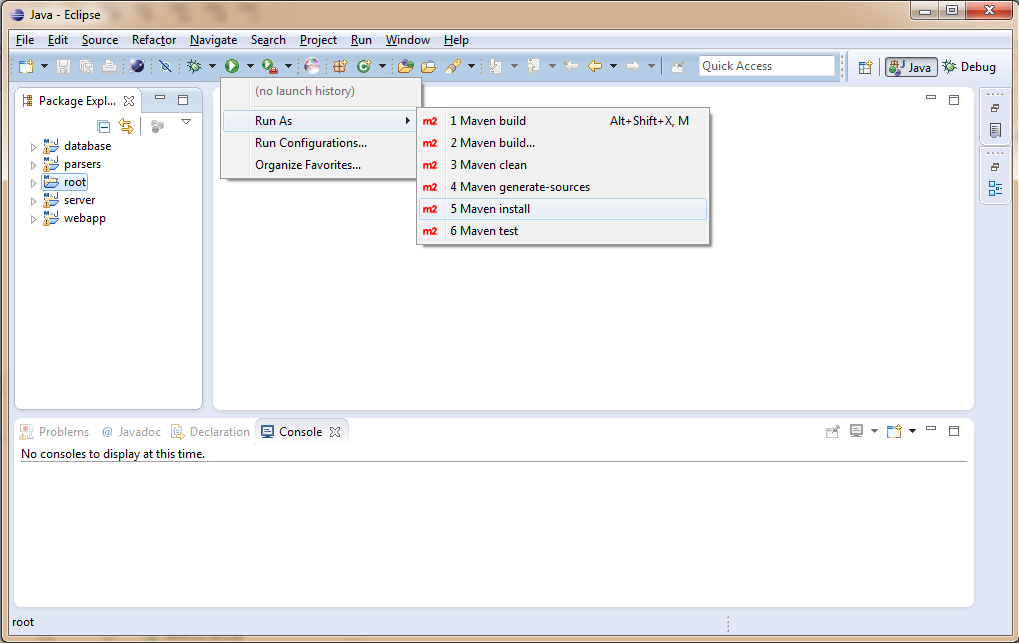
\includegraphics[width=1.1\textwidth]{../img/fvcN51B.png}
\caption{Eclipse Maven install run}
\label{run03}
\end{figure}


\begin{figure}[htbp]
\centering
  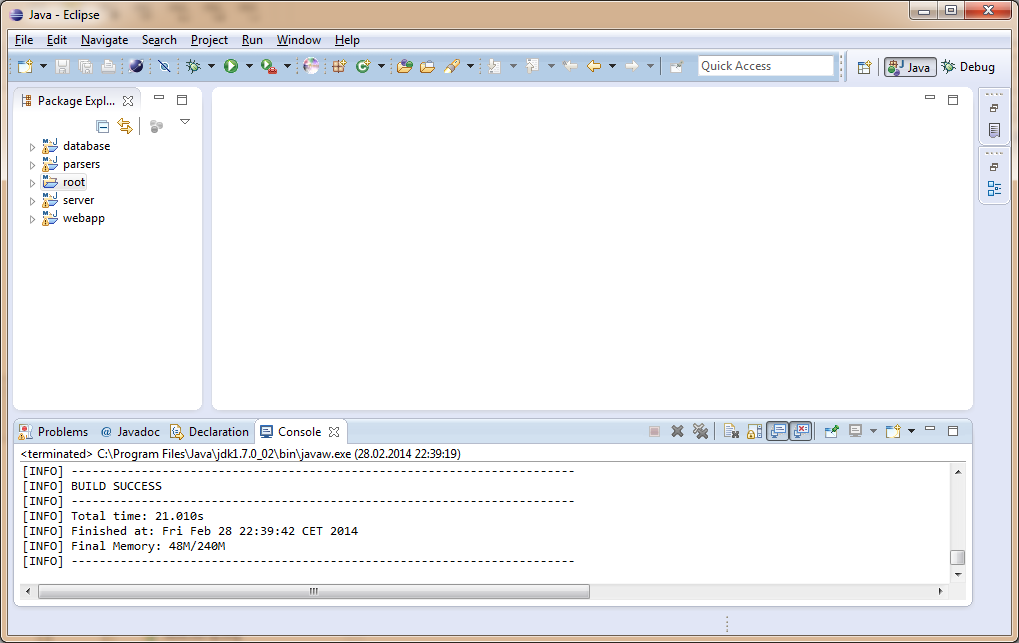
\includegraphics[width=1.1\textwidth]{../img/v13HHJO.png}
\caption{Eclipse Maven build successfuly}
\label{run04}
\end{figure}
  
  
\begin{figure}[htbp]
\centering
  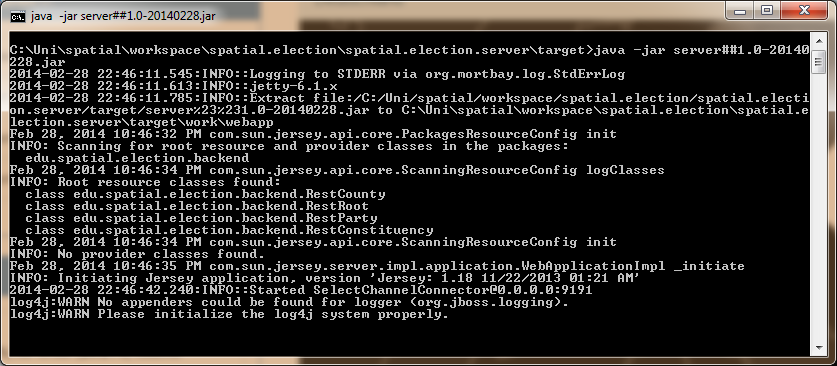
\includegraphics[width=1.1\textwidth]{../img/wFn3GVG.png}
\caption{Java execution of the project binary}
\label{run05}
\end{figure}

\begin{center}\rule{3in}{0.4pt}\end{center}


\subsection{Running a build war file with
Tomcat}\label{running-a-build-war-file-with-tomcat}

\begin{enumerate}
\def\labelenumi{\arabic{enumi}.}
\itemsep1pt\parskip0pt\parsep0pt
\item
  Follow the same steps from the previous part: Run the ``Install''
  command, wait for the ``BUILD SUCCESS'' message in the console.
\item
  Go to the ``server'' subproject directory, navigate to target. There
  you should find a war file. Import this file to your tomcat server.
  Usually its administration GUI is available from
  ``{[}\ldots{}{]}/manager/html/''.
\item
  After importing the war file, you should be able to click the link
  ``Spatial Election'' in the list of Tomcat applications. It will guide
  you to the project website.
\end{enumerate}

\end{document}
